\documentclass[../main.tex]{subfiles}
\graphicspath{{\subfix{../figures/}}}
%
\title{读书笔记}
%
\begin{document}
\maketitle
\begin{cuenotes}
  \cue{为什么要做读书笔记}
  \note{
    很多人读了一本书书像没读过一样,很大的一个原因在于,
    他们没有记读书笔记的习惯。而良好的笔记习惯,是提高读书效率的关键。
    \begin{itemize}
      \item \textbf{转被动阅读为主动阅读}:
        大部分人的阅读是一种被动获取信息的方式,
        这是一种比较低效的学习方式。
        而做读书笔记能让你从被动的阅读转变为主动的思考,
        激发大脑的积极性。
      \item \textbf{加深对关键概念的理解}:
        记笔记的过程是一个将知识进行压缩和内化的过程。
        把几十万字的书,压缩成几页文字或一张思维导图,
        这个过程不仅让你抓住了书本中的重点,
        还促进了你对关键概念的理解。
      \item \textbf{梳理逻辑结构和主线}:
        当你阅读完一本书时,可以问自己一个问题``这本书讲了些什么''。
        如果你能很好地把握住文章的主线,理清书里的逻辑结构,
        那么这个问题对你来说并不难。
      \item \textbf{温故知新,加深记忆}:
        能做到过目不忘的人是天赋异禀,
        正常人看完一本书最难以避免的就是遗忘。
        人的记忆容量有限,做读书笔记是加深理解和记忆的有效途径。
        此外,更方便后续的回顾和随时检索,常记常新。
    \end{itemize}
  }
  \cue{几种读书笔记方法}
  \note{
    \begin{itemize}
      \item \hyperlink{摘录式笔记法}{摘录式笔记法}
      \item \hyperlink{批注式笔记法}{批注式笔记法}
      \item \hyperlink{康奈尔笔记法}{康奈尔笔记法}
      \item \hyperlink{大纲式笔记法}{大纲式笔记法}
      \item \hyperlink{思维导图笔记法}{思维导图笔记法}
    \end{itemize}
  }
  \cue{\hypertarget{摘录式笔记法}{摘录式笔记法}}
  \note{
    阅读时,可以把喜欢的描写或者认为重要的内容按照原文进行抄录。
    抄录时,能加深对文段的印象。很多人可以对读过的书进行旁征博引,
    信手拈来,用的就是这种方法。虽然看似简单,但当你做足了量的积累,
    在写文章或论文时却非常有用。 \\
    摘录式笔记很重要的一点是注明原文出处,页数和作者,以便引用和查询。
  }
  \cue{\hypertarget{批注式笔记法}{批注式笔记法}}
  \note{
    批注式笔记法是在书中标记重要内容的基础上,
    在空白处加上相关的联想和注释。这种笔记方法的优势在于其便利性,
    你可以边读边记,一边标注出对你有用的关键内容,
    一边记录下你的所思所想。 \\
    批注的内容可以多样,不管是字词句的理解,还是关键概念引发的思考,
    还是此时此地的想法,或是联想的相关案例都可以。
    应用的场景也很多元,不管是文学类书籍的阅读,还是专业的著作,
    都可采用这种方式。 \\
    批注式和摘录式笔记的共同优点是简单,但缺点也很明显,
    这两种笔记方式都是比较被动的笔记方式。
    这两种笔记方式对知识是``浅层次''的加工(或者说没有加工),
    不涉及信息的压缩和提取,后续对知识的记忆和提取贡献程度也有限。
  }
  \cue{\hypertarget{康奈尔笔记法}{康奈尔笔记法}}
  \note{
    康奈尔笔记法,又叫 5R 笔记法:
    \begin{itemize}
      \item 记录(Record):在听讲或阅读过程中,
        在主栏内尽量多记有意义的论据、概念等讲课内容。
      \item 简化(Reduce):下课以后,尽可能及早将这些论据、
        概念简明扼要地概括(简化)在回忆栏,即副栏。
      \item 背诵(Recite):把主栏遮住,只用回忆栏中的摘记提示,
        尽量完满地叙述课堂上讲过的内容。
      \item 思考(Reflect):将自己的听课随感、意见、经验体会之类的内容,
        与讲课内容区分开,写在卡片或笔记本的某一单独部分,
        加上标题和索引,编制成提纲、摘要,分成类目。并随时归档。
      \item 复习(Review):每周花十分钟左右时间,快速复习笔记,
        主要是先看回忆栏,适当看主栏。
    \end{itemize}
    其实简单来说就是在白纸上画三条线,
    来区分\emph{上课/阅读时},\emph{上课/阅读后},\emph{复习时}三个时间阶段各自需要做的事情。
    如下图:
  }
  \note{
    \begin{figure}[H]
      \begin{center}
        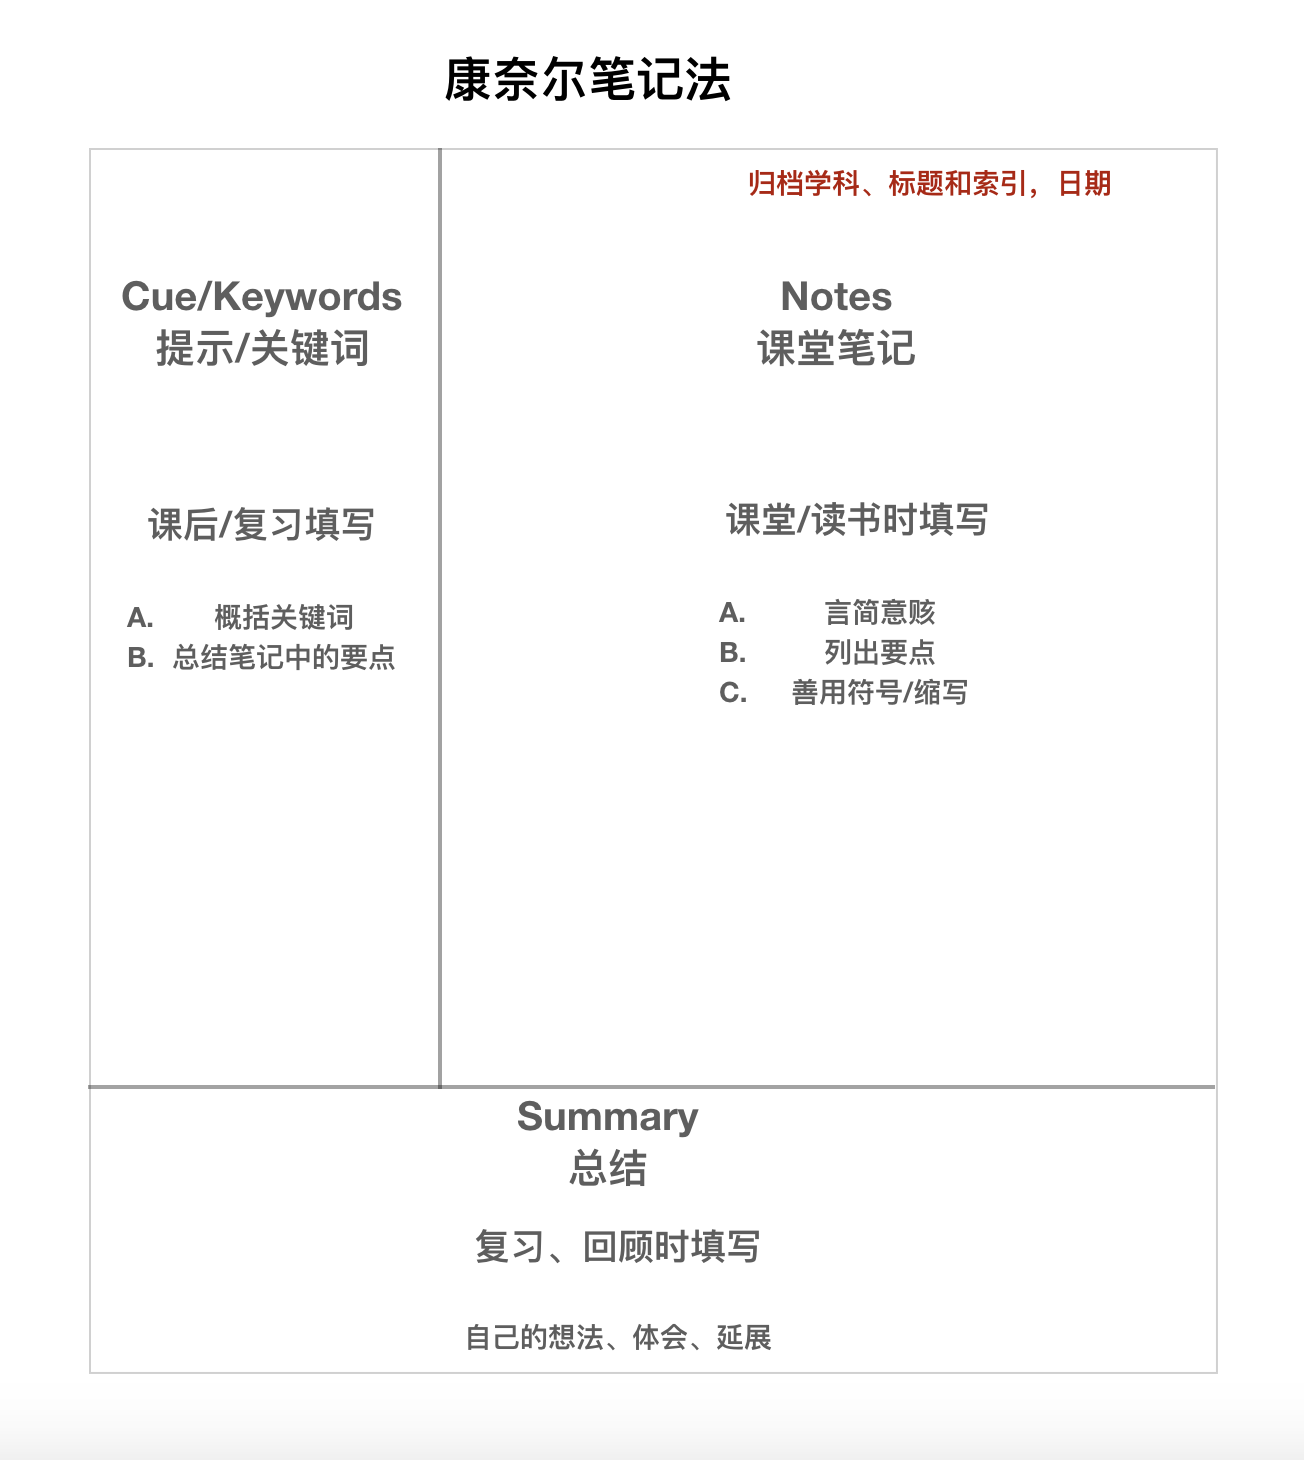
\includegraphics[width=0.80\textwidth]{cornell_note.png}
      \end{center}
      \caption{康奈尔笔记模板}
    \end{figure}
  }
  \note{
    用这种方法记笔记,最大的好处就是很好地利用了记忆曲线,
    并有效加强理解和记忆。让你主动去进行关键词的提取,并及时回忆,
    加强你对听课/阅读内容的理解。
  }
  \note{
    这种笔记方式非常适合课堂和具体章节的复习,
    因为每一节课讲的内容比较细分。但这种笔记方式也有缺点,
    一是它的内容承载量比较小,讨论的层面会比较窄且具体,
    不适用于构架知识框架。二是它的拓展性较差,当你有新的知识汇入时,
    很难在原有的笔记上进行拓展。
  }
  \cue{\hypertarget{大纲式笔记法}{大纲式笔记法}}
  \note{
    大纲是结构化的笔记。当我们对书本的关注重点不仅局限于某一个部分,
    而是想从整体上对整本书的整体框架和逻辑结构有一定的把握时,
    可以熟练运用大纲式笔记法。
    在书本目录的基础上,用大纲的方式将书本的内容进行压缩和呈现,
    起到一个提纲挈领的作用。体系化笔记的好处在于,非常有利于复习。
    当你在进行课程复习,或者回想读过的内容时,可以边看笔记边进行回想。
  }
  \note{
    这种笔记方式可以结构清晰地按照总分关系对所读的内容进行归纳和整理。
    但大纲笔记在某些程度上是受限制的,比如说除了总分关系外,
    它没有办法表达节点之间的相互联系,所能承载的元素也有限。
  }
  \note{
    \begin{figure}[H]
      \begin{center}
        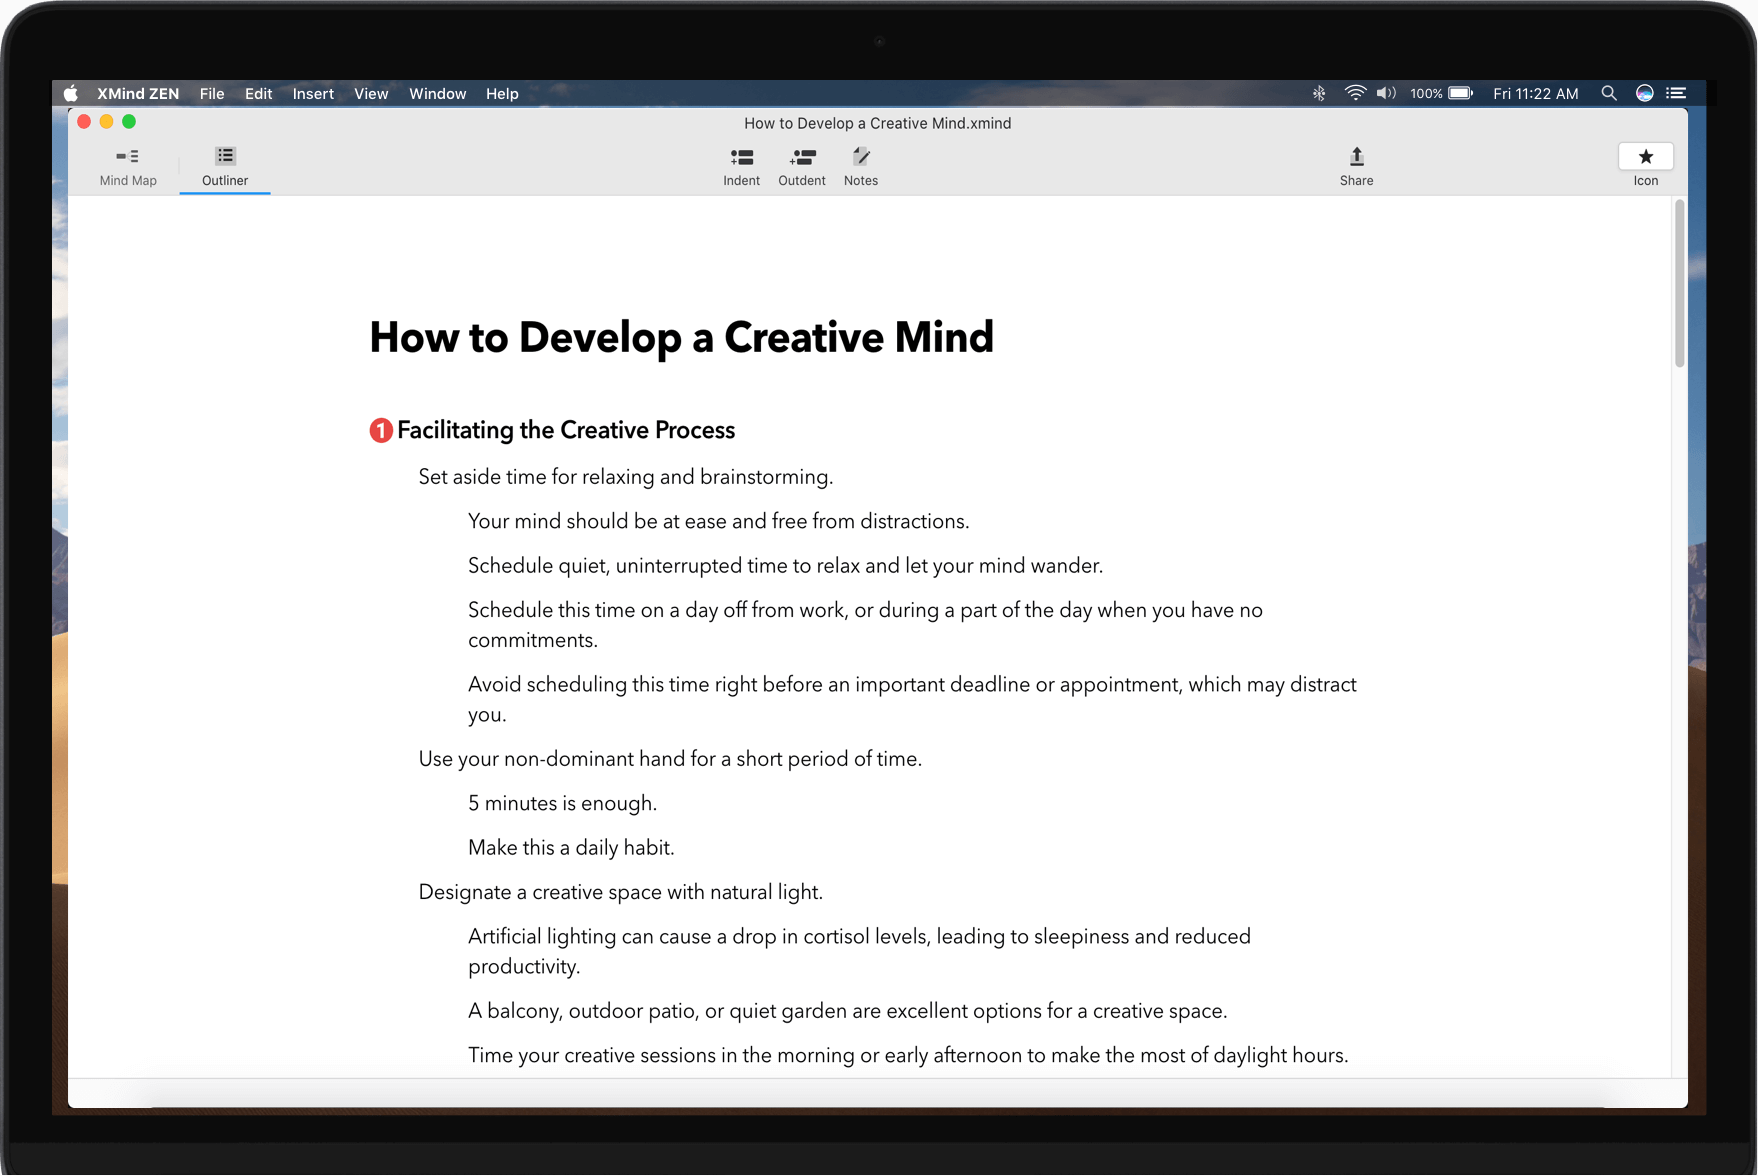
\includegraphics[width=0.95\textwidth]{outline_note.png}
      \end{center}
      \caption{大纲式笔记法}
    \end{figure}
  }
  \cue{\hypertarget{思维导图笔记法}{思维导图笔记法}}
  \note{
    思维导图是用一个中央关键词或想法引起形象化的构造和分类的想法;
    它用一个中央关键词或想法以辐射线形连接所有的代表字词、想法、
    任务或其它关联项目。
    思维导图的笔记方式对知识是``深层次''加工,
    绘制思维导图相当于是对信息重新进行编码,
    这种加工方式更有利于记忆和理解。
    因为你要对接收的信息进行压缩,不断地进行关键词的提取,
    分类、总结概括,类比,发散,找出知识间的内在逻辑。
    通过树形结构把知识进行串联,在搭建结构的时候,
    每增加一个主题分支就是一次新的思考和连接。
    在记笔记的过程中,大脑是高度积极参与的。
  }
\end{cuenotes}
%
\end{document}
